\documentclass[conference]{IEEEtran}


%\usepackage{cite}

% *** GRAPHICS RELATED PACKAGES ***
%
\ifCLASSINFOpdf
  \usepackage[pdftex]{graphicx}
  \usepackage{epstopdf}
  %\usepackage[demo]{graphicx}
  % declare the path(s) where your graphic files are
  \graphicspath{{./fig/}}
  % and their extensions so you won't have to specify these with
  % every instance of \includegraphics
  \DeclareGraphicsExtensions{.pdf,.jpeg,.png}
\else
  % or other class option (dvipsone, dvipdf, if not using dvips). graphicx
  % will default to the driver specified in the system graphics.cfg if no
  % driver is specified.
  \usepackage[dvips]{graphicx}
  % declare the path(s) where your graphic files are
  % \graphicspath{{../eps/}}
  % and their extensions so you won't have to specify these with
  % every instance of \includegraphics
  % \DeclareGraphicsExtensions{.eps}
\fi
% graphicx was written by David Carlisle and Sebastian Rahtz. It is
% required if you want graphics, photos, etc. graphicx.sty is already
% installed on most LaTeX systems. The latest version and documentation can
% be obtained at: 
% http://www.ctan.org/tex-archive/macros/latex/required/graphics/
% Another good source of documentation is "Using Imported Graphics in
% LaTeX2e" by Keith Reckdahl which can be found as epslatex.ps or
% epslatex.pdf at: http://www.ctan.org/tex-archive/info/
%
% latex, and pdflatex in dvi mode, support graphics in encapsulated
% postscript (.eps) format. pdflatex in pdf mode supports graphics
% in .pdf, .jpeg, .png and .mps (metapost) formats. Users should ensure
% that all non-photo figures use a vector format (.eps, .pdf, .mps) and
% not a bitmapped formats (.jpeg, .png). IEEE frowns on bitmapped formats
% which can result in "jaggedy"/blurry rendering of lines and letters as
% well as large increases in file sizes.
%
% You can find documentation about the pdfTeX application at:
% http://www.tug.org/applications/pdftex





% *** MATH PACKAGES ***
%
\usepackage[cmex10]{amsmath}
\usepackage{mathtools}
\usepackage{gensymb}
% A popular package from the American Mathematical Society that provides
% many useful and powerful commands for dealing with mathematics. If using
% it, be sure to load this package with the cmex10 option to ensure that
% only type 1 fonts will utilized at all point sizes. Without this option,
% it is possible that some math symbols, particularly those within
% footnotes, will be rendered in bitmap form which will result in a
% document that can not be IEEE Xplore compliant!
%
% Also, note that the amsmath package sets \interdisplaylinepenalty to 10000
% thus preventing page breaks from occurring within multiline equations. Use:
%\interdisplaylinepenalty=2500
% after loading amsmath to restore such page breaks as IEEEtran.cls normally
% does. amsmath.sty is already installed on most LaTeX systems. The latest
% version and documentation can be obtained at:
% http://www.ctan.org/tex-archive/macros/latex/required/amslatex/math/





% *** SPECIALIZED LIST PACKAGES ***
%
\usepackage{algorithmic}
% algorithmic.sty was written by Peter Williams and Rogerio Brito.
% This package provides an algorithmic environment fo describing algorithms.
% You can use the algorithmic environment in-text or within a figure
% environment to provide for a floating algorithm. Do NOT use the algorithm
% floating environment provided by algorithm.sty (by the same authors) or
% algorithm2e.sty (by Christophe Fiorio) as IEEE does not use dedicated
% algorithm float types and packages that provide these will not provide
% correct IEEE style captions. The latest version and documentation of
% algorithmic.sty can be obtained at:
% http://www.ctan.org/tex-archive/macros/latex/contrib/algorithms/
% There is also a support site at:
% http://algorithms.berlios.de/index.html
% Also of interest may be the (relatively newer and more customizable)
% algorithmicx.sty package by Szasz Janos:
% http://www.ctan.org/tex-archive/macros/latex/contrib/algorithmicx/


% *** ALIGNMENT PACKAGES ***
\usepackage{array}
\usepackage{multirow}
% Frank Mittelbach's and David Carlisle's array.sty patches and improves
% the standard LaTeX2e array and tabular environments to provide better
% appearance and additional user controls. As the default LaTeX2e table
% generation code is lacking to the point of almost being broken with
% respect to the quality of the end results, all users are strongly
% advised to use an enhanced (at the very least that provided by array.sty)
% set of table tools. array.sty is already installed on most systems. The
% latest version and documentation can be obtained at:
% http://www.ctan.org/tex-archive/macros/latex/required/tools/


%\usepackage{mdwmath}
%\usepackage{mdwtab}
% Also highly recommended is Mark Wooding's extremely powerful MDW tools,
% especially mdwmath.sty and mdwtab.sty which are used to format equations
% and tables, respectively. The MDWtools set is already installed on most
% LaTeX systems. The lastest version and documentation is available at:
% http://www.ctan.org/tex-archive/macros/latex/contrib/mdwtools/


% IEEEtran contains the IEEEeqnarray family of commands that can be used to
% generate multiline equations as well as matrices, tables, etc., of high
% quality.


%\usepackage{eqparbox}
% Also of notable interest is Scott Pakin's eqparbox package for creating
% (automatically sized) equal width boxes - aka "natural width parboxes".
% Available at:
% http://www.ctan.org/tex-archive/macros/latex/contrib/eqparbox/





% *** SUBFIGURE PACKAGES ***
%\usepackage[tight,footnotesize]{subfigure}
% subfigure.sty was written by Steven Douglas Cochran. This package makes it
% easy to put subfigures in your figures. e.g., "Figure 1a and 1b". For IEEE
% work, it is a good idea to load it with the tight package option to reduce
% the amount of white space around the subfigures. subfigure.sty is already
% installed on most LaTeX systems. The latest version and documentation can
% be obtained at:
% http://www.ctan.org/tex-archive/obsolete/macros/latex/contrib/subfigure/
% subfigure.sty has been superceeded by subfig.sty.



%\usepackage[caption=false]{caption}
%\usepackage[font=footnotesize]{subfig}
% subfig.sty, also written by Steven Douglas Cochran, is the modern
% replacement for subfigure.sty. However, subfig.sty requires and
% automatically loads Axel Sommerfeldt's caption.sty which will override
% IEEEtran.cls handling of captions and this will result in nonIEEE style
% figure/table captions. To prevent this problem, be sure and preload
% caption.sty with its "caption=false" package option. This is will preserve
% IEEEtran.cls handing of captions. Version 1.3 (2005/06/28) and later 
% (recommended due to many improvements over 1.2) of subfig.sty supports
% the caption=false option directly:
%\usepackage[caption=false,font=footnotesize]{subfig}
%
% The latest version and documentation can be obtained at:
% http://www.ctan.org/tex-archive/macros/latex/contrib/subfig/
% The latest version and documentation of caption.sty can be obtained at:
% http://www.ctan.org/tex-archive/macros/latex/contrib/caption/




% *** FLOAT PACKAGES ***
%
%\usepackage{fixltx2e}
% fixltx2e, the successor to the earlier fix2col.sty, was written by
% Frank Mittelbach and David Carlisle. This package corrects a few problems
% in the LaTeX2e kernel, the most notable of which is that in current
% LaTeX2e releases, the ordering of single and double column floats is not
% guaranteed to be preserved. Thus, an unpatched LaTeX2e can allow a
% single column figure to be placed prior to an earlier double column
% figure. The latest version and documentation can be found at:
% http://www.ctan.org/tex-archive/macros/latex/base/



\usepackage{stfloats}
% stfloats.sty was written by Sigitas Tolusis. This package gives LaTeX2e
% the ability to do double column floats at the bottom of the page as well
% as the top. (e.g., "\begin{figure*}[!b]" is not normally possible in
% LaTeX2e). It also provides a command:
%\fnbelowfloat
% to enable the placement of footnotes below bottom floats (the standard
% LaTeX2e kernel puts them above bottom floats). This is an invasive package
% which rewrites many portions of the LaTeX2e float routines. It may not work
% with other packages that modify the LaTeX2e float routines. The latest
% version and documentation can be obtained at:
% http://www.ctan.org/tex-archive/macros/latex/contrib/sttools/
% Documentation is contained in the stfloats.sty comments as well as in the
% presfull.pdf file. Do not use the stfloats baselinefloat ability as IEEE
% does not allow \baselineskip to stretch. Authors submitting work to the
% IEEE should note that IEEE rarely uses double column equations and
% that authors should try to avoid such use. Do not be tempted to use the
% cuted.sty or midfloat.sty packages (also by Sigitas Tolusis) as IEEE does
% not format its papers in such ways.





% *** PDF, URL AND HYPERLINK PACKAGES ***
%
\usepackage{url}
% url.sty was written by Donald Arseneau. It provides better support for
% handling and breaking URLs. url.sty is already installed on most LaTeX
% systems. The latest version can be obtained at:
% http://www.ctan.org/tex-archive/macros/latex/contrib/misc/
% Read the url.sty source comments for usage information. Basically,
% \url{my_url_here}.


%\usepackage{hyperref}


% *** Do not adjust lengths that control margins, column widths, etc. ***
% *** Do not use packages that alter fonts (such as pslatex).         ***
% There should be no need to do such things with IEEEtran.cls V1.6 and later.
% (Unless specifically asked to do so by the journal or conference you plan
% to submit to, of course. )


% correct bad hyphenation here
\hyphenation{op-tical net-works semi-conduc-tor}
\usepackage{ bbold }
\usepackage[utf8]{inputenc}
\DeclareUnicodeCharacter{00A0}{~}
\newcommand\PoP{\mathit{PoP}}
\newcommand\VNF{\mathit{VNF}}
\newcommand\CEO{\mathit{C_{or}}}
\newcommand\SVNF{\mathit{SvNF}}


\begin{document}

\title{Migrating to a NFV-based Home Gateway: introducing a Surrogate vNF approach}



\author{\IEEEauthorblockN{Nicolas Herbaut}
\IEEEauthorblockA{Viotech Communications \\
CNRS, LaBRI Lab.,\\
Université de Bordeaux\\
Talence, France\\
nicolas.herbaut@labri.fr}
\and
\IEEEauthorblockN{Daniel Negru}
\IEEEauthorblockA{CNRS, LaBRI Lab.,\\
Université de Bordeaux\\
Talence, France\\
daniel.negru@labri.fr}
\and
\IEEEauthorblockN{George Xilouris}
\IEEEauthorblockA{NCSR Demokritos\\
Athens, Greece\\
xilouris@iit.demokritos.gr}
\and
\IEEEauthorblockN{Yiping Chen}
\IEEEauthorblockA{Orange Labs\\
Issy-les-moulineaux, France\\
yiping.chen@orange.com}
}



\maketitle


\begin{abstract}
Virtualizing network functions is becoming a major trend in today's research on cloud computing.
Among networking elements, the Home Gateway appears to be one with the most diverse functions to handle and thus, with great potential for virtualization.
To this end, the paper proposes a solution to ease adoption by Service Providers of the latest breakthroughs in cloud computing technologies towards a virtualized Home Gateway.
Although the NFV approach globally pretends bringing operational advantages in terms of CAPEX and OPEX, it is essential to prove them for Home Gateways scenarios where compatibility and versatility are strong requirements. To achieve this goal, we introduce the concept of Surrogate vNF, which makes Home Gateways NFV aware.
The paper highlights a migration path towards full Home Gateway virtualization and proves its concept through a real implementation and a simulated evaluation on a practical use case related to video content distribution.
\end{abstract}

\begin{IEEEkeywords}
Home Gateway, Network Function Virtualization, OSGI
\end{IEEEkeywords}



\IEEEpeerreviewmaketitle



\section{Introduction \label{sec:introduction}}

\begin{figure*}
  \begin{center}
    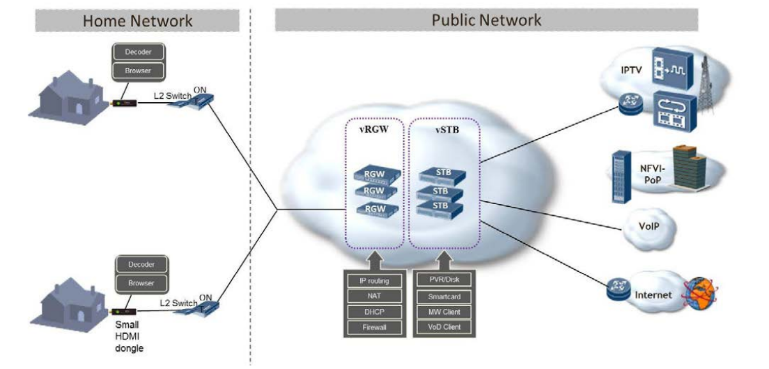
\includegraphics[width=0.90\textwidth,natwidth=769,natheight=369]{fig/vHGetsi.png}
  \end{center}
  \caption{ Virtualization of the home environment according to ETSI.
    \label{fig:etsi-vision}
  }
\end{figure*}

Since the introduction of high speed Internet technologies such as xDSL and FTTx, End-Users' demands for Internet services grow at an exponential rate.
According to Akamai, the most popular Content Delivery Network (CDN) provider, the average bandwidth has continued to globally increase by 65\% in the second quarter of 2014 \cite{_akamais_2014} compared to 2013.

More interestingly, Akamai's report mentions that the share of users having sufficient bandwidth to stream 4K/Ultra HD has doubled in 2014, globally reaching 10\% of the connected users.
This format represents a minimal resolution of 3840x2160 pixels or 15Mbp/s for a video encoded with a regular H.264/MPEG-4 AVC codec.
By the time of writing, there's a limited amount of 4K ready Set Top Boxes due to hardware limitations (e.g. compute power, HDMI version).

Once IP packets arrived at the customer's premises, they are processed by equipments such as Home Gateways (HG) and Set-Top Boxes (STB), to deliver content to a number of devices such as screens, smartphones, tablets, computers, mobile devices and security appliances.
HG and STB are placed on the last portion of the Service Provider's (SP) network under the conjoined responsibility of the End-User (EU) and the SP.
Functionally, the HG consists of the modem part that assures the translation of layers 1 and 2 between two heterogeneous networks: the SP's access network and the EU's home network.
For more advanced cases, it also handles higher level operations on network and transport layer by performing for example Network Address Translation (NAT).
The STB device is responsible for allowing access to IP video streamed services on their TV, such as live TV or Video On Demand (VOD).
It is also responsible for transcoding the content currently received as a MPEG-2 or MPEG-4 stream to an uncompressed media format such as HDMI or analog signal.

Furthermore, HG \& STB usually consist of self-contained components, using internally stored firmware.
When new configuration updates are released, new model and firmware upgrades are being constantly pushed to the market.
The hardware and software fragmentation becomes more and more prominent, increasing operational expenses (OPEX). 

In the highly competitive industry of SP, where the arrival of a new player can be a game changer, new services and new norms are frequently rolled out.	
The impact on Customer Premise Equipment (CPE), like HG or STB, can be huge, as software updates can be insufficient to cover new requirements.
Updating hardware is vital, however this leads to high capital expenditure (CAPEX).
For instance, most STBs cannot decode the new video format standard  High Efficiency Video Coding (HEVC).
This is due to the fact that the current decoders (H.264) have been implemented using hardware chips not covering HEVC or that they have insufficient compute power to do it in software (empirical tests performed in \cite{grois_performance_2013} have shown that HEVC encoding is 18x slower than H264).

The challenge for SP is twofold: they must find a way to tackle with disruptive changes brought by the fast apparition of new technologies driven by E.U. new expectations (like adopting 4K or 8K TV) while lowering expenses induced by replacing their network hardware.

Cloud Computing (largely surveyed in the literature as in \cite{rimal_taxonomy_2009}) has been both a hype and a game changer for the IT industry for nearly a decade.
It allows innovation to be deployed on commodity servers, contributing to the rapid expansion of Software-as-a-Service like messaging software or social networks, offering scalability, fault tolerance and interoperability.
Initially powered only by proprietary solutions like Amazon Web Services\footnote{http://aws.amazon.com/} for cloud infrastructure and Google Cloud Platform\footnote{https://cloud.google.com} for cloud platform, free and open source software are gaining further importance notably through the OpenStack\footnote{http://www.openstack.org/} project. 

The missing steps to provide the power of Cloud Computing to SP Operational and Business Support Services (OSS/BSS) is a well-defined network architecture along with a normalization effort and vendor-supported building blocks.

Drawing on this observation, the European Telecommunications Standards Institute (ETSI) issued a seminal white paper \cite{_network_2012}, introducing the notion of Network Function Virtualization (NFV) and launched an Industry Specification Group for NFV, producing frequent publications.
The NFV concept aims at creating a reference architecture and a standardized approach to achieve carrier grade virtualization of existing hardware middle boxes on commodity servers.
Network equipment vitalization touches a broad range of devices, including HG and STB as ETSI mentions in the “Virtualization of the Home Environment” section of \cite{_network_2013}. 

As interest in NFV grows, several field studies are performed to verify it can be launched to market.
However, the transition from the current monolithic firmware based CPE to a proper full cloud solution is unlikely to happen immediately.

In this paper, we will study the feasibility of a NFV based HG. We propose a Virtual Network Function (VNF) integrated into a HG that will serve as a drop-in replacement for an existing function by leveraging the usage of Open Services Gateway initiative (OSGi\footnote{http://www.osgi.org/}) technology, for seamless HG exploitation within the cloud.

The rest of this paper is organized as follows.
Section II, will focus on the current and next generation Home Gateway architectures.
Section III will review existing approaches for visualizing CPEs in general.
Section IV will be dedicated to the description of our proof of concept, for which experimentations and results will be discussed in Section V.
Finally, Section VI will conclude and introduce future work.




\section{Background and related work \label{sec:background}}

%Even if historically customers still think they are connected to the Internet using a simple modem, the truth is that broadband connection is delivered by a full-fledged HG, integrating the functions of a modem, network address translation (NAT) router, Ethernet switch, WiFi access point, DHCP server, firewall, among others.
 
No standard technical specification has been defined for HG. However a set of Functional Requirements is maintained by the Broadband Forum in TR-124 \cite{broadband_forum_functional_2014}.
The following section will present the most common architectures for HGs.
A special interest will be shown for execution environments, which are meant to achieve modularity through the Service Oriented Programming (SOP) paradigm \cite{bieber2001introduction}.


\subsection{Architecture and execution environment for HG}

\subsubsection{Firmware based HG}
HG's firmware is a custom proprietary embedded system software deployed by vendors into their devices.
This solution is still widely used by vendors, but lacks the ability to act as a real execution environment.
Even if Service Providers or End-Users can alter its configuration, new services cannot easily be deployed on-the-fly.
A complete system update by the Service Providers is necessary to deploy new features.
   
\subsubsection{GNU/Linux HG}
   
GNU/Linux is also used as a platform of choice for Home Gateways \cite{royon_multiservice_2007}.
The solution is considered stable, tested and allows reusing well-known applications for networking, among others.
After Linksys (a router vendor who published its GNU/Linux based firmware designed for its WRT54G product line in 2003), a lot of efforts have been made to maintain and improve embedded GNU/Linux firmware distribution over a wide variety of platforms.

A notable example is the OpenWrt\footnote{https://openwrt.org/} project which has been partly sponsored among others by Comcast, through the Open Home Gateway Forum.
It has helped researchers to add new features to commodity routers by replacing the firmware with a real GNU/Linux OS along with a file system and a package management tool.
In addition of being able to deploy new packaged programs, developers can also use OpenWrt to write their own applications and deploy them in production.


Modularity can be achieved within the GNU/Linux platform.
The large application catalog available, usually benefits from low memory consumption and low IO footprint.
However, programs must be cross platform and Service Oriented Architecture is not natively supported.
Due to this, alternative execution environments such as OSGi are promoted.


   
\subsubsection{HG with OSGI execution environment}
   
OSGi is a specification that describes a modular system and a service platform for Java.
It was originally designed to enable the deployment of services over wide area networks to local networks and devices (\cite{marples_open_2001}).
The main advantages of OSGI are platform and application independency, multiple services support and collaboration by letting services discovering each other and adapting their behaviour accordingly.

The Home Gateway Initiative (HGI)\footnote{http://www.homegatewayinitiative.org} publishes Requirements \cite{_requirements_2011} \cite{_hg_2014} proposing an architecture for Modular HG.
It explicitly indicates OSGi as the solution of choice to deploy additional modules in their HGI Open Platform 2.0.
This deals with the modularity issues of the latter approaches.
For HGI, the goal for OSGi is to allow the installation, update, removal, start and stop of new software component leaving the underlying firmware image untouched.

\subsubsection{Alternative execution environements}

A new trend in CPE design has emerged conjointly with the availability of alternative opensource OSes like Android\footnote{among others Bbox Miami, Freebox mini 4K are built with Android TV OS}.
Rich of hundred thousands third party applications, they bring directly to the end-user the possibility of installing additional software to enrich the user exeperience.
Another advantage for this model is that End-Users are already familiar with the concept of application store, and their willingness to pay extra for services and applications has risen with the smartphone era.
For the Internet Service Providers the advantage is the great professional support available for those OSes, easying maintenance and support and also the possibility to agree on revenue sharing\footnote{http://www.bloomberg.com/news/articles/2014-10-02/orange-agrees-to-distribute-netflix-video-service-in-france} with over the top (OTT) content providers like Netflix or Canal+.

Even if Android comes from the smartphone world, the platform have a good support for SOP, with the service abstraction, sandboxing and built-in security. Multi-vendor services and applications can be installed and their lifecycle support the most common traits of a service bundle with the help of the built-in Task Scheduler.

\begin{figure*}
  \begin{center}
    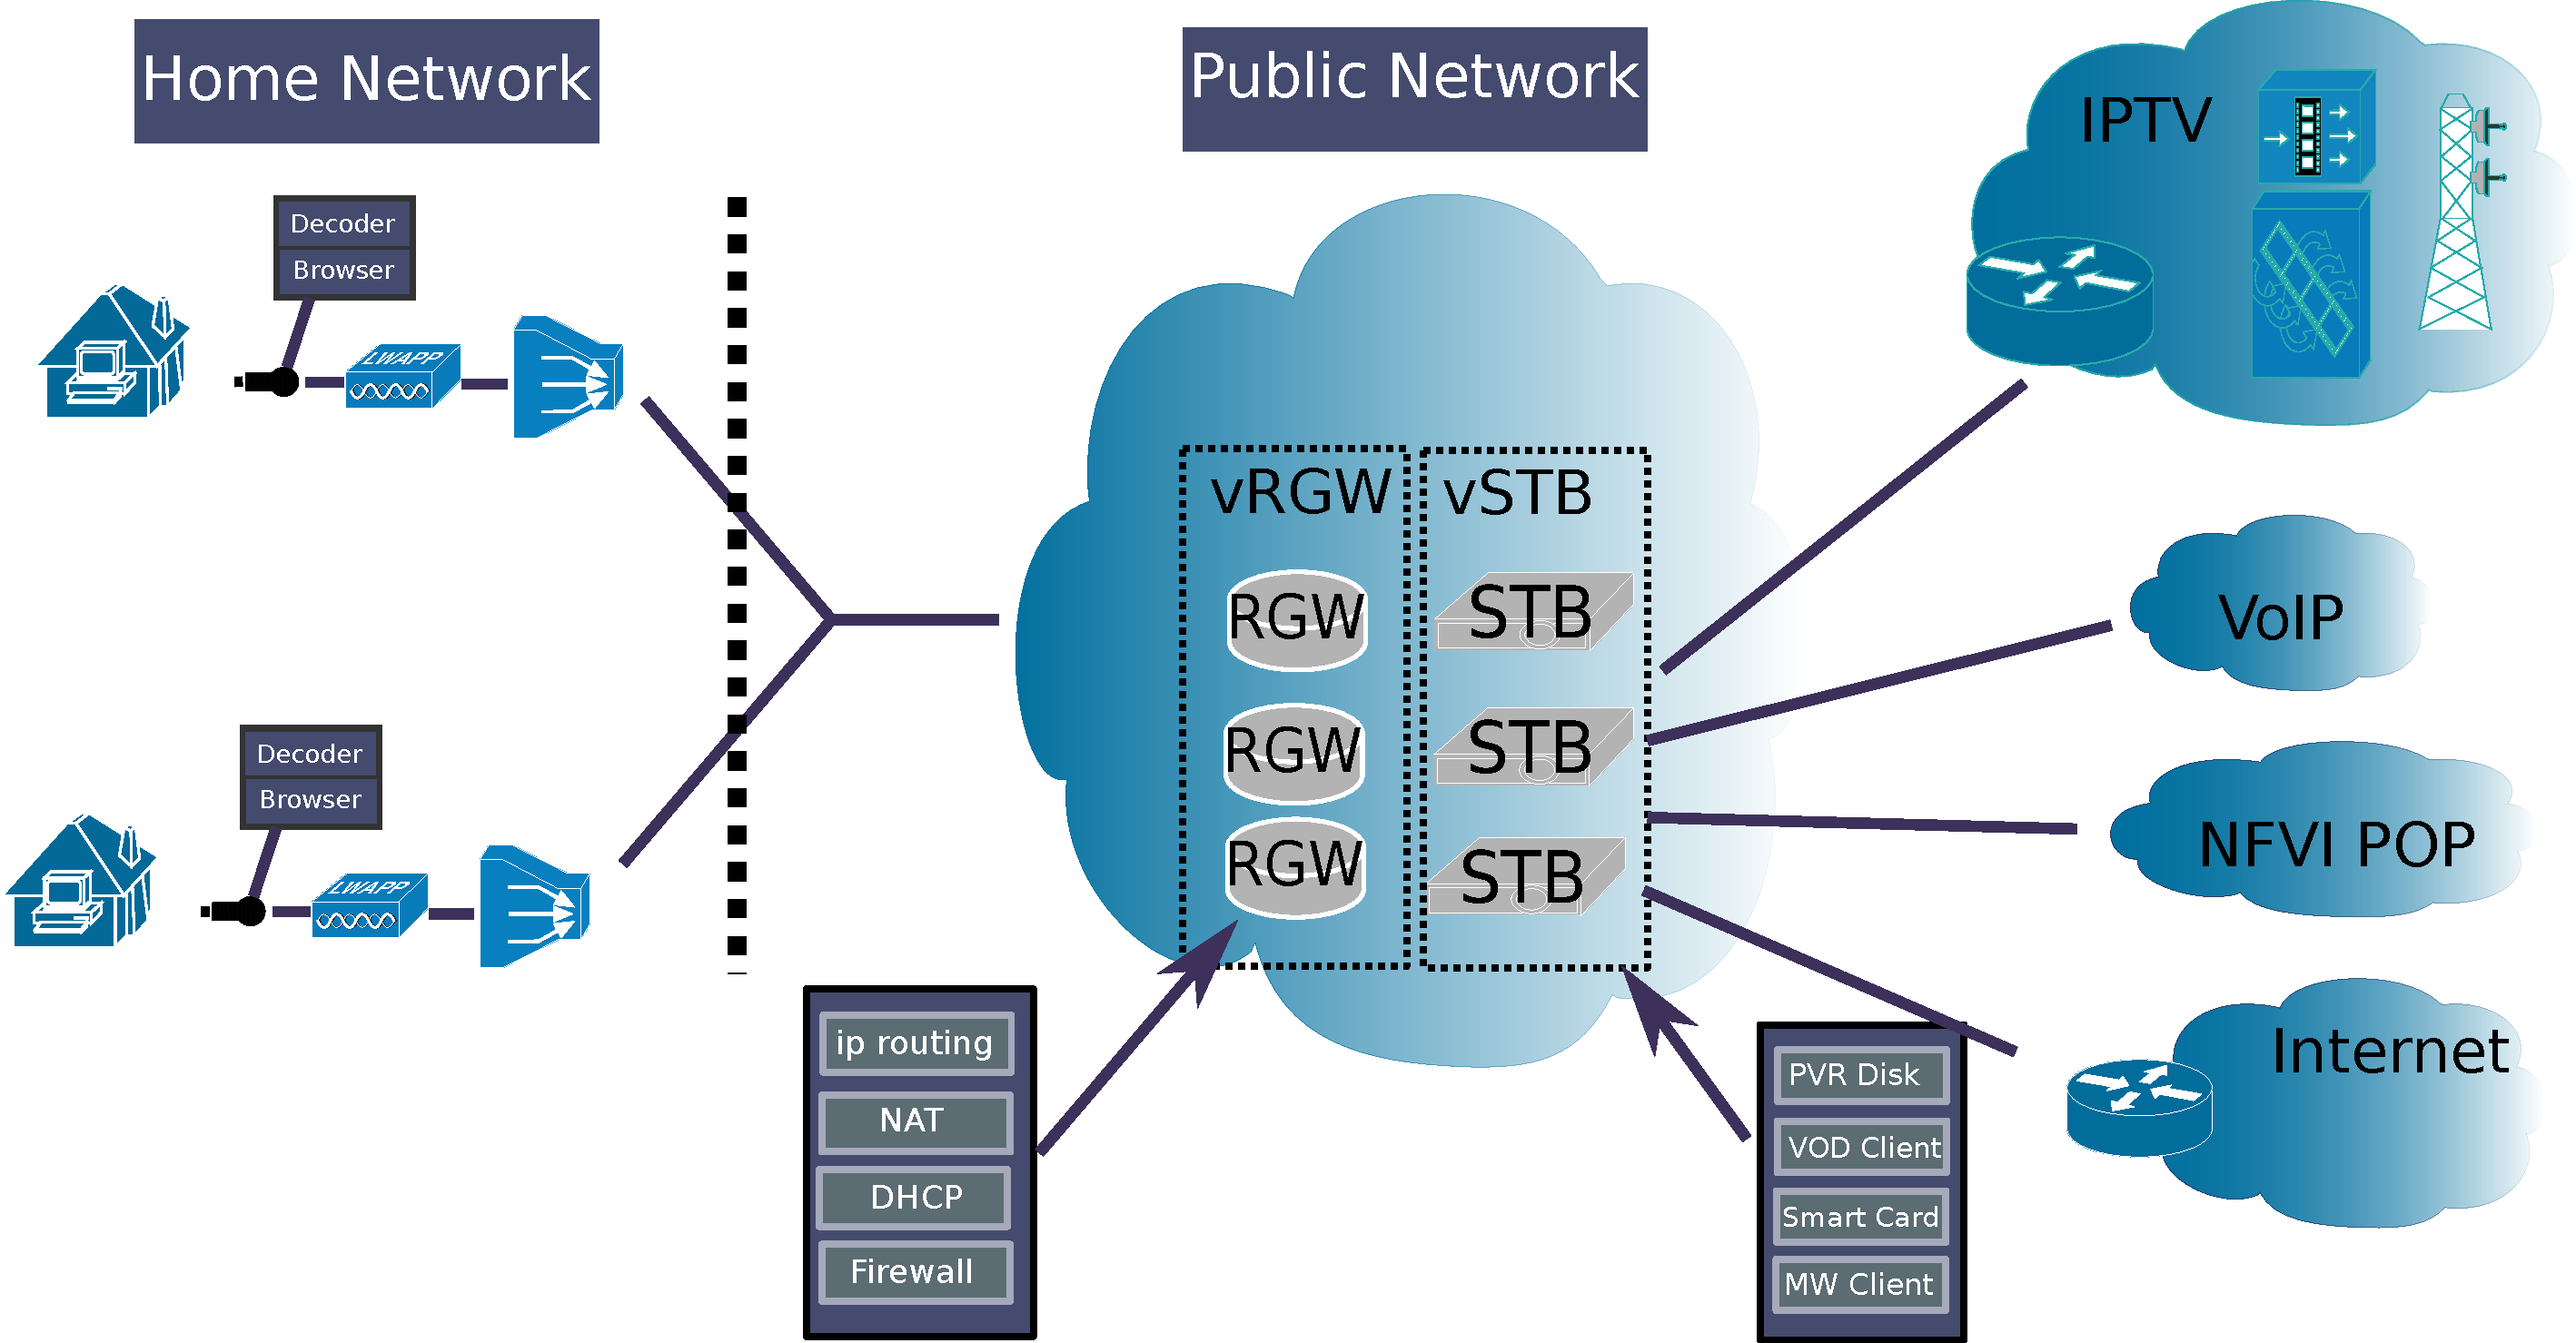
\includegraphics[width=0.9	\textwidth]{fig/etsi-virtualisation-home-env.pdf}
  \end{center}
  \caption{ Virtualisation of the home environment according to ETSI.
    \label{fig:etsi-vision}
  }
\end{figure*}


\subsection{Home Gateway Virtualisation}
The idea of virtualizing Home Gateways is not new.
Being a disruptive technological change, proposing new architecture is a challenging task.
It involves a great understanding of Service Providers access networks specificities, architecture choices, legacy and limitations.
The opportunity of virtualizing HG is often coupled with the adoption of new technology such as fibre, since it allows new network capabilities and by dropping legacy twisted pair physical layer.

The study from Eurescom \cite{daniel_abgrall_virtual_????} starts by describing existing standards from the Broadband Forum and assuming deployment scenarios for a vHG.
By replacing existing HG with a managed bridge, Service Providers would replace the current HG with a simplified layer-2 device having the ability to manage VoIP and WiFi interfaces.
In the study, Software Defined Network (SDN) is also proposed to tackle scalability issues arising from integrating a significant number of vHG instances on network equipments.
By proposing a software architecture related to the HGI proposal to deploy network function in a modularized fashion, they suggest the principle of NFV architecture.
It is also claimed that the current Broadband Forum standards allow support of vHG even if its architecture is not defined, leaving the way open to using NVF.

In \cite{da_silva_home_2011} authors qualitatively compare several architectures for HG virtualisation (which in this case is merely layer-2 based home and access network with Plug and Play capabilities), explaining that it could be achieved (among other proposals) by centralizing the virtual routing [network] function (specially NAT) in the broadband remote access server.
This method requires significant changes in the SP access network.

In \cite{cruz_architecture_2013} Cruz et al demonstrates a proposal built upon two reference frameworks from the Broadband forum (TR-101 and TR-156), which shows vHG being deployed in SP datacenter as embedded GNU/Linux virtual machines managed by the CWMP protocol to simplify management on the SP side.

In \cite{_network_2013} ETSI build out its proposal for using vNF in virtualizing the home environment over Eurescom work, by setting the vHG as a virtualisation target, as show in Figure~\ref{fig:etsi-vision}.
Benefits for this architecture include both CAPEX and OPEX reduction as well as improved QoE through remote access and multi-screen support.
The introduction of new services without dependencies on the CPE capabilities is also outlined.
In this scenario, the full stack of the HG and STB functionalities are moved to the cloud, leaving only simple Level-2 bridges in the customer's premises.
They mention that SP is likely to roll out virtualized services gradually based on available access technology and End User requirements, without specifying the technical way to integrate both worlds.
The paper is trying to address this main issue.

In \cite{lee_netserv:_2011} authors propose to revive Active Networking by designing a framework allowing SP or Content Providers (CP) to deploy new functionalities on the network in a secure and dynamic fashion.
NetServ Controller exposes packets to OSGi bundles for packet processing.

\begin{figure}
  \begin{center}
    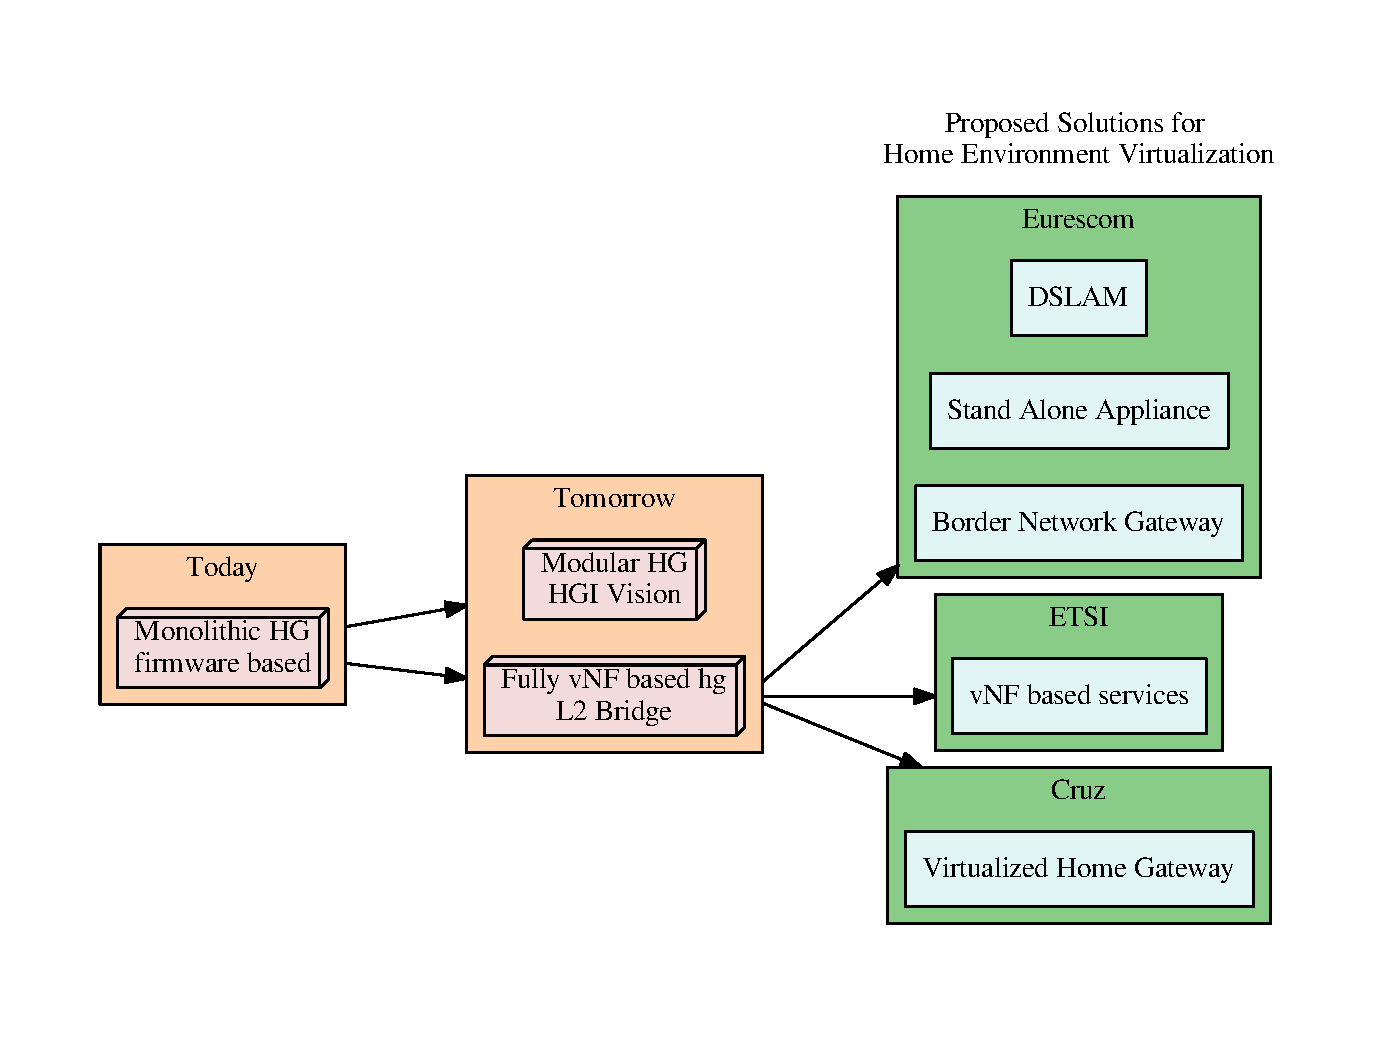
\includegraphics[width=0.45\textwidth]{fig/vhgtrends.pdf}
  \end{center}
  \caption{ Major trends for technical aspects of Home Gateway Virtualisation
    \label{fig:trends}
  }
\end{figure}	
Figure~\ref{fig:trends} sums up the most relevant trends for the next generation HG which were previously discussed.
Building up on the latter approaches, this paper investigates an alternate, yet standard-based, migration path to a fully virtualized home environment, centred around a modular HG (using HGI open platform 2.0 with OSGi) cooperating with a carrier grade cloud computing architecture (NFV-ready and ETSI compliant).






\section{Migrating to a NFV-based home gateway \label{sec:migrating} using a Surrogate VNF approach}

\begin{figure}
  \begin{center}
    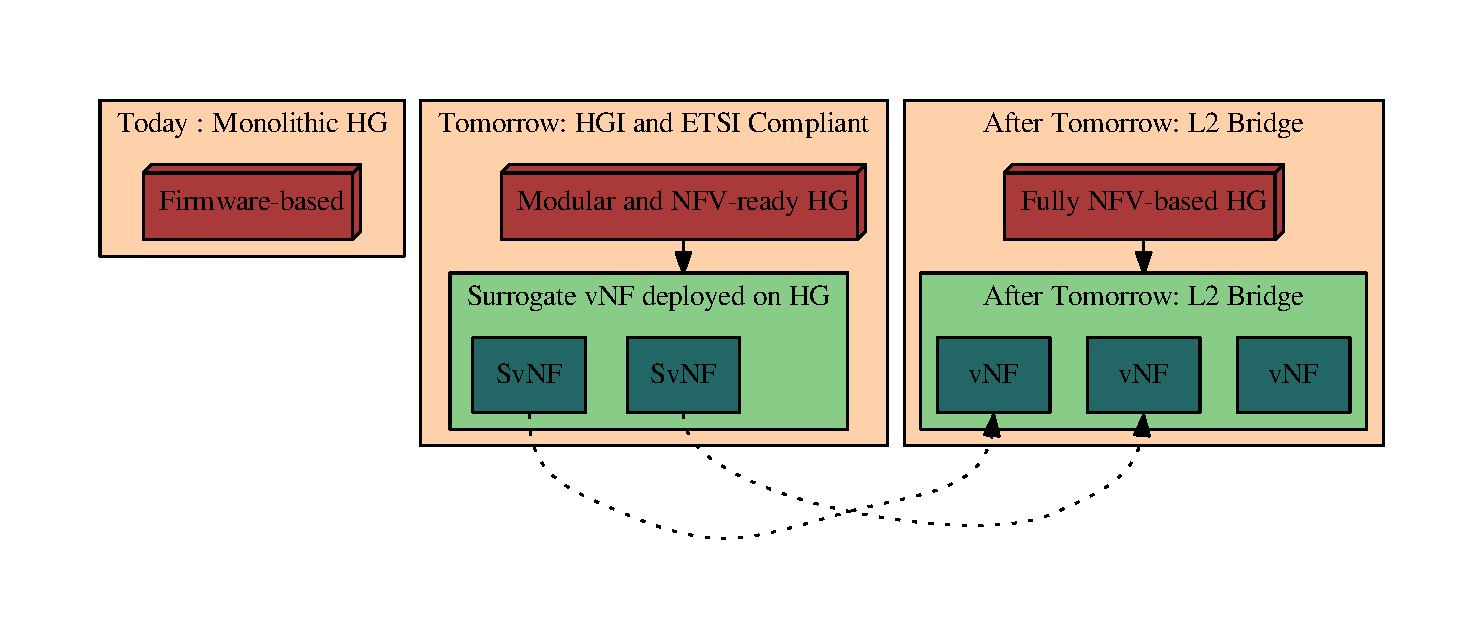
\includegraphics[width=0.45\textwidth]{fig/migrationPath.pdf}
  \end{center}
  \caption{ Migration path from Modular to Virtual HG.
    \label{fig:migration}
  }
\end{figure}	

\begin{figure*}
	
	\center

	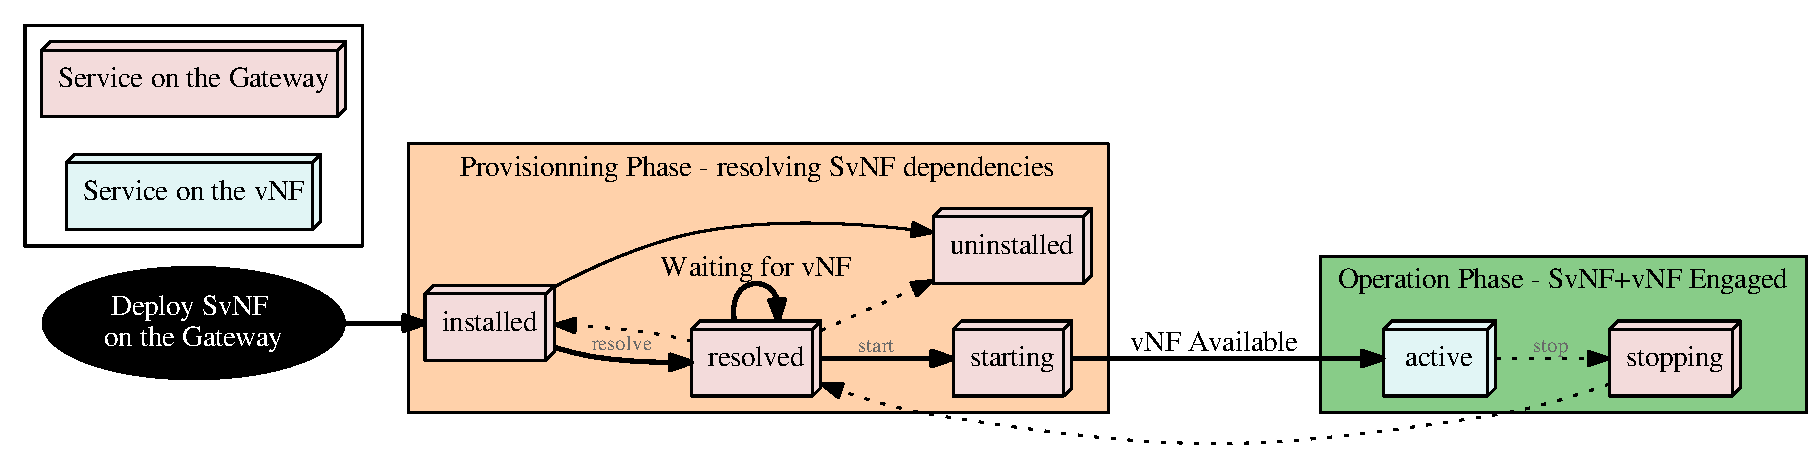
\includegraphics[width=0.90\textwidth]{fig/osgi.pdf}
	\caption{ Supporting SvNF operation using standard OSGi life cycle.
    \label{fig:osgisvnf}
    }

\end{figure*}
	   

Given all the advantages brought by the virtualisation of the home environment, we should see a dramatic market swap.
Even if field studies are currently conducted\footnote{Telefónica and NEC win innovation award for virtualized home gateway trials: http://tinyurl.com/o8cl3bv}, they focus mainly on emerging markets.
For more mature markets, SPs balance those advantages with the necessity to dampen their past investments made on their current infrastructures.
There is also a technological risk in building VHG infrastructure at scale, especially in a deflationary market where investments need to take opportunistic pathes. 

Focusing on the introduction of \textit{new services} made possible by virtualisation techniques has the advantage of not beeing too disturbing for the current infrastructure, while paving the way for a future migration to a full fledge virtual environment. Our proposal is to demonstrate that with the current infrastrusture, we can integrate NFV within the gateways to deploy new services easily.

\subsection{The Surrogate vNF Concept}





We propose an alternative migration path where vNFs collaborate with modular gateways. We introduce the concept of \textit{Surrogate vNF} (SvNF) in Figure~\ref{fig:migration}. 
A SvNF is an OSGi bundle that acts like a regular module from the HG standpoint, except that it delegates any significant operation to a vNF.

The key role played by the SvNF+vNF couple in the migration path is that the vNF part is used on both the OSGi modular gateway scenario and on the L2 bridge scenario, allowing gradual migration of SP installed based while securing investments of the vNF. 

SvNF modules leverage the existing OSGi lifecycle and resource provisionning mechanisms, but extend it also to network resources. SvNF modules are aware of SP access network capabilities to support vNFs, so they can be registered in the HG OSGi execution environment only if they are supported by the underlying network.
As shown in ~Figure \ref{fig:osgisvnf}, we extend the semantics of OSGi lifecycle by adding the capability to depend on network resources as well. SvNF modules register themselves on the runtime environement only if any suitable vNF is available to them. The HG falls back to legacy mode and keep using the native implementation of the service if the virtualized one is not available.

Using SvNF, SPs are able to push new services to every customers in an hybrid scenario where some customers go 100\% virtualized where it makes sense, while the others still run their legacy home gateways

 
\subsection{Feasibility: application to video delivery}
\begin{figure*}
	
	\center

	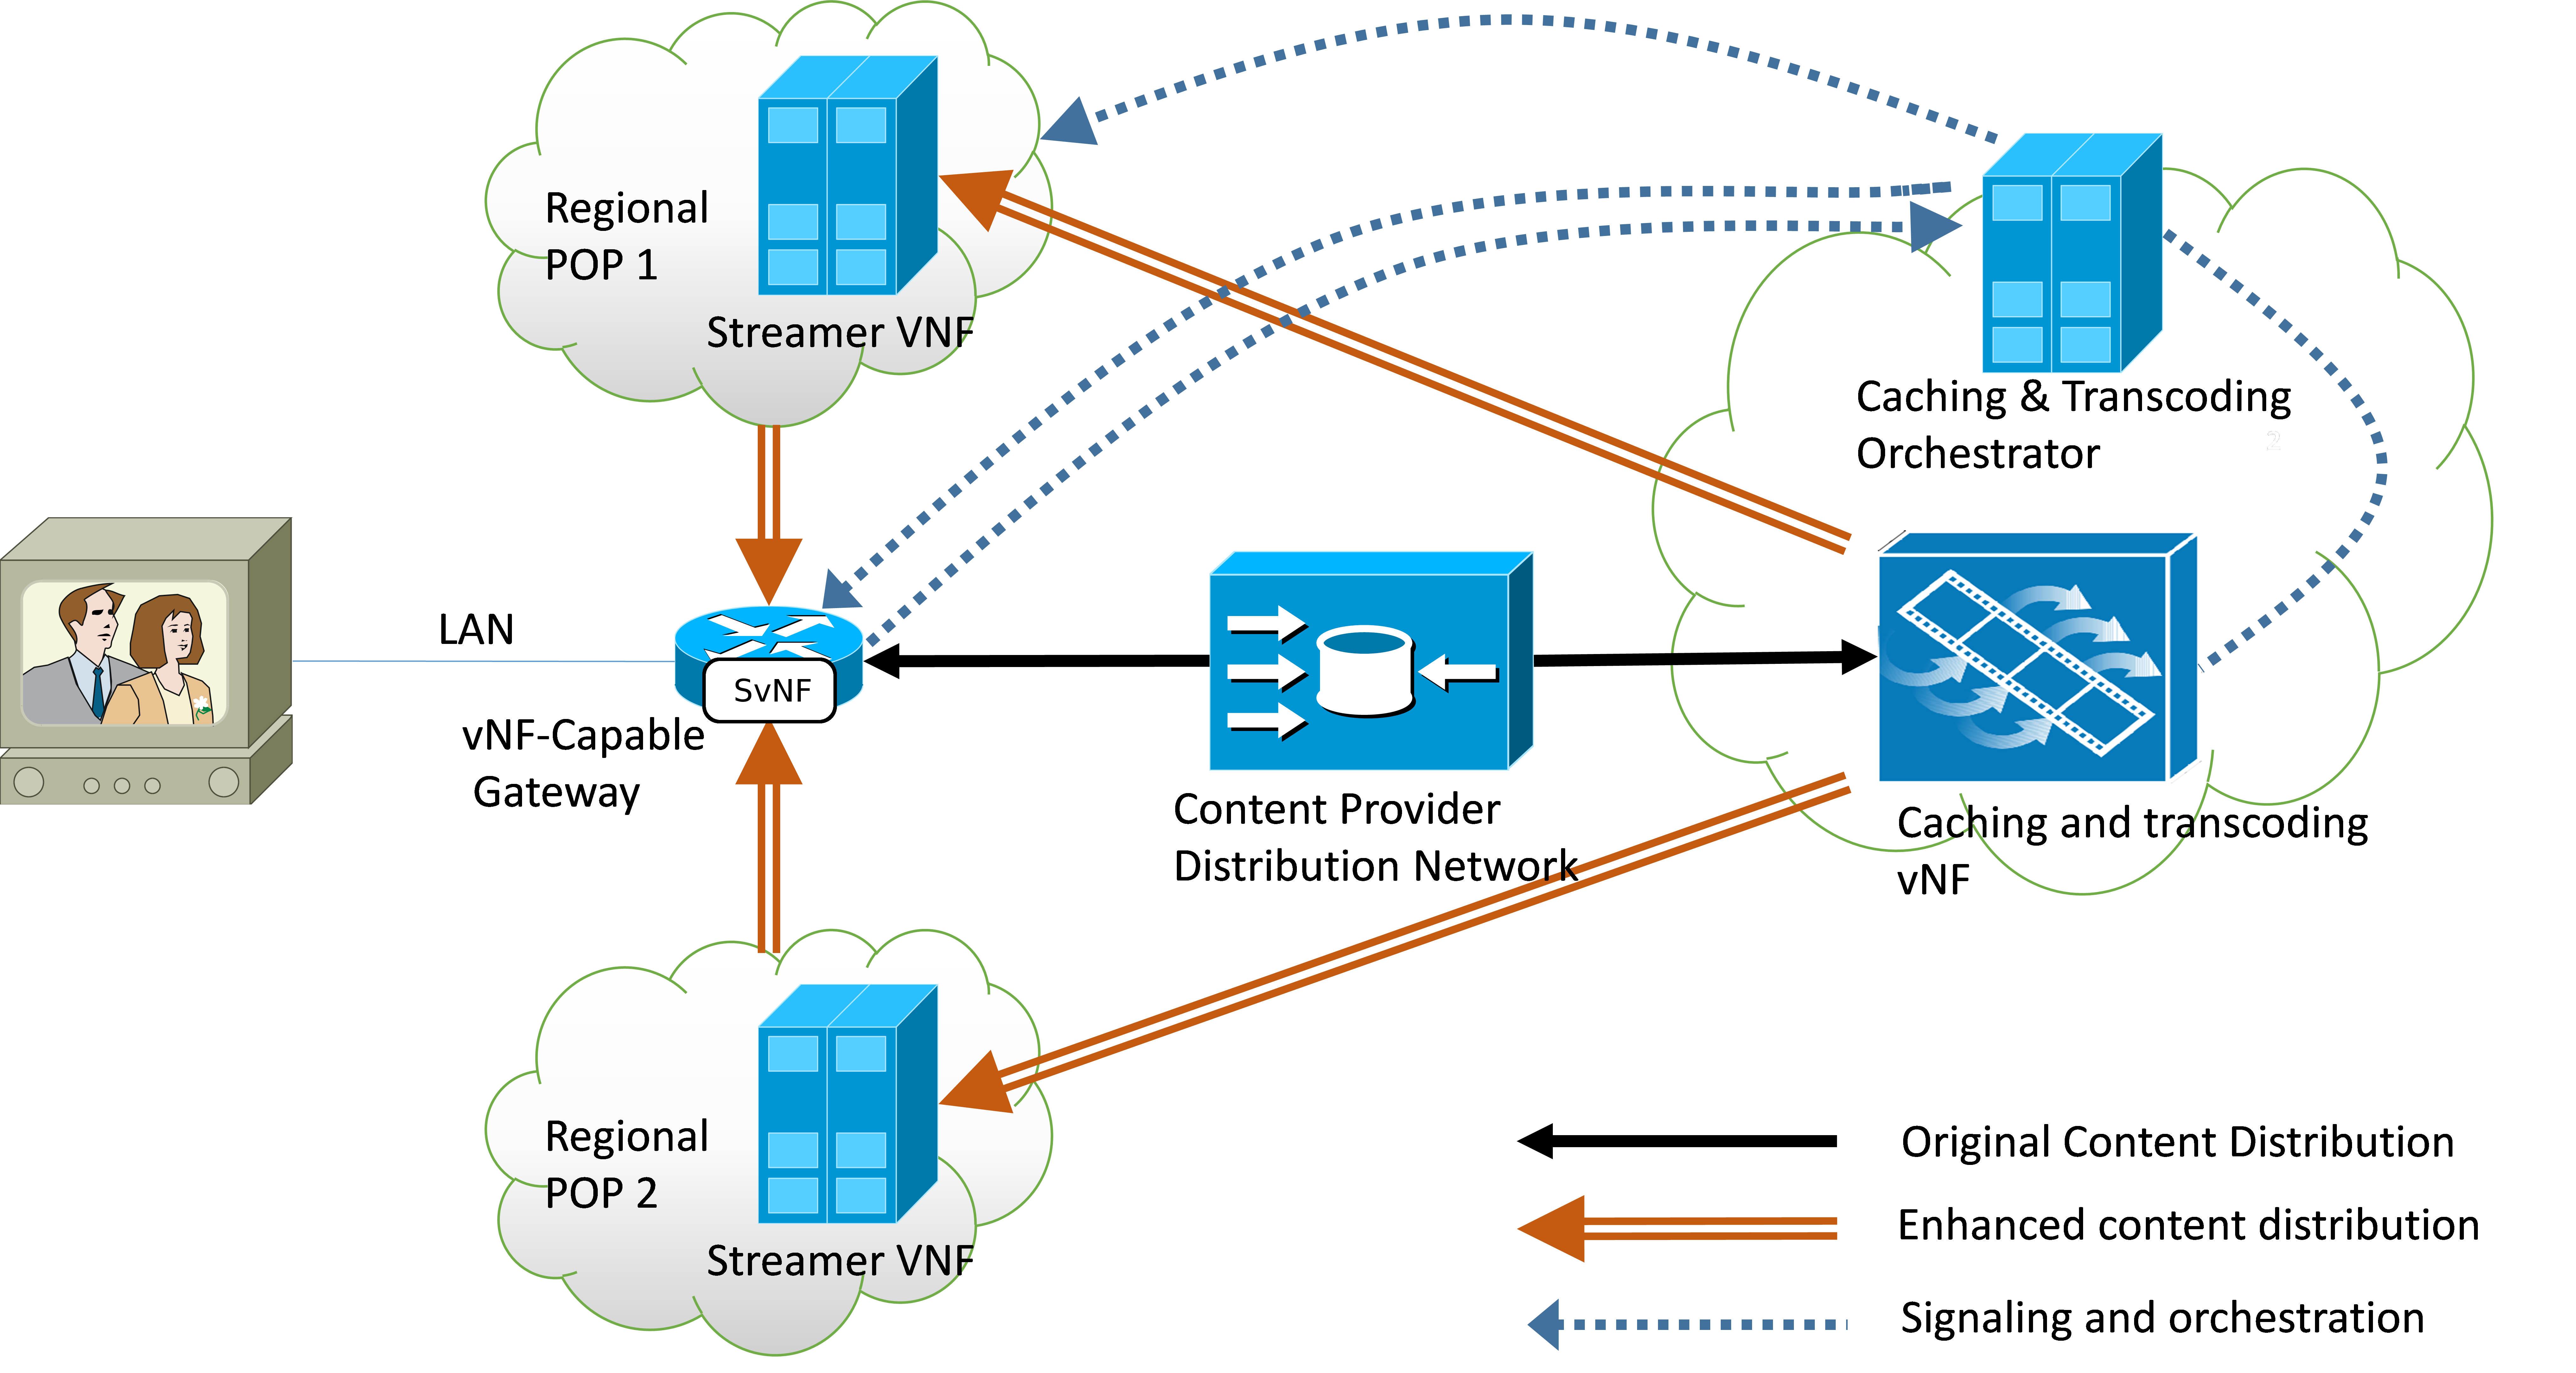
\includegraphics[width=0.90\textwidth,natwidth=8132,natheight=4335]{fig/highleveldesign.png}
	\caption{ High level design
    \label{fig:hld}
    }

\end{figure*}

To demonstrate the feasibility of a modular and NFV-ready HG, we realized a proof of concept (POC).
In order for this POC to be highly relevant, we had to consider the best possible Network Functions to be virtualised.
We could have focused on core functions such as DHCP or NAT, which are challenging to virtualize at scale. However, virtualizing them doesn't illustrate how \textit{new services and features} could be rolled out easily on the gateway.

We thus decided to highlight the advantages of our proposal by deploying a new type of SvNF+vNF related to multimedia that improves the End-User's Quality of Experience related to video consumption and enhance network performances at the same time.
Such a function can be introduced into a modular OSGi HG and its execution would definitely be efficient as a vNF, due to the heavy video processing tasks it involves.


The use case consists of an End User $u$ consuming media from his Set-Top Box, connected to his HG where the $\SVNF_{u}$ is running.
Video streams of a VOD or IPTV service are transferred from the content provider distribution network \(\mathit{CP}_{\mathit{network}}\) (which may or may not include Content Delivery Networks - CDNs) to the TV and across $\SVNF_{u}$.
Figure~\ref{fig:hld} depicts the design of the system and the use case steps. The figure presents the interactions between CP, SP and End-User for a classical video streaming use case.
In the original content distribution model, content is streamed from the content provider network  to the user gateway \(\SVNF_{u}\).

Classic deployment scenario involve the use of content distribution network to offload the CP main server.
CDN nodes are often collocated with internet exchange points (IXP) which present the advantage of being located relatively close of the End-User. Our use case however, presents an alternative model where the content is cached in a regional point of presence managed by the SP (also called micro-data centers located at the edge of the network). The content delivered by a streaming vNF deployed in the POP.

The caching and encoding orchestrator  $\CEO$ maintains a list of provisioned of regional POPs \(\POP=\{p_{i}\}\) that can handle cache requests. On each $p_{i}$ is deployed a set of Streaming vNF that serve content to users.

$\CEO$ also manages gateway configuration. It pushes a set of rules \(R_{u}=\{r^{u}_{1},r^{u}_{2},...,r^{u}_{n}\}\) on the $\SVNF_{u}$. 
Those rules are used to filter requests and responses crossing $\SVNF_{u}$ in order to notify the $\CEO$ that a video is requested.
It also pushes a list of cached resources available to $\SVNF_{u}$ through the POPS $C_{u}=\{c^{i,u}_{j} \}$ where $j$ is the identifier of the resource and $i$ the identifier of the POP $p_{i}$ from which it can be retreived.

The SvNF module deployed on the HG works as a HTTP proxy.
When it receives a request from client or a response from a server, it analyses it using the set of rules \(R_{u}\) and the set of cached resource $C_{u}$ deployed on the HG.
Depending on the result several scenarios can occur.
Let's consider the three possible scenarios.

%\paragraph{Step1}EU requests the content from the vNF-Capable Gateway. 
%\paragraph{Step 2}
%The vNF-Capable Gateway analyses the video format, and checks it is technically compatible with the system (e.g. a supported video codec and supported delivery method).
%If it is compatible, we continue to scenario 2, otherwise, we proceed with scenario 1.

\subsubsection*{Scenario 1: no operation scenario}\label{noop}

In this scenario, the content consumed by the user is not eligible to the enhancements brought by the system. None of the rules $r_{i}$ deployed on $\SVNF_{u}$ matches the request or the response and and the content doesn't match any $c^{i,u}_{j}$ either. We note $\mathbb{1}_{r_{i}}(.)$ and $\mathbb{1}_{c^{i,u}_{j}}(.)$ such that:
\[
    \mathbb{1 }_{r_{i}}(\mathit{message})= 
\begin{dcases}
    1& \text{if rule $r_{i}$ matches the message} \\
    0              & \text{otherwise}
\end{dcases}
\]
and 
\[
    \mathbb{1 }_{c^{i,u}_{j}}(\mathit{resource})= 
\begin{dcases}
    1& \text{if rule $c^{i,u}_{j}$ matches the resource} \\
    0              & \text{otherwise}
\end{dcases}
\]

After the gateway has analysed the request, it is forwarded to its original destination.

\begin{algorithmic}[1]
	
\STATE User $u$ requests a resource
\STATE $\SVNF_{u}$ receives request $\mathit{Req}$ from $u$
\STATE \( \sum_{r^{u}_{i}\in R_{u}}{\mathbb{1}_{r_{i}}(\mathit{Req})}=0 \)
\STATE \( \sum_{c^{i,u}_{j}\in C_{u}}{\mathbb{1}_{c^{i,u}_{j}}(\mathit{Req})}=0 \)
\STATE $\SVNF_{u}$ forward $\mathit{Req}$ to its original target \(\mathit{CP}_{\mathit{network}}\)
\STATE $\SVNF_{u}$ receives response $\mathit{Res}$ from \(\mathit{CP}_{\mathit{network}}\)
\STATE \( \sum_{r^{u}_{i}\in R_{u}}{\mathbb{1}_{r_{i}}(\mathit{Res})}=0 \)
\STATE User $u$ receives $\mathit{Res}$ from \(\mathit{CP}_{\mathit{network}}\) through $\SVNF_{u}$
\end{algorithmic}


The content is then directly consumed by the End-User from the Content Provider Delivery Network.
This is the common case, as it is performed today. The HG does not bring any added value to the consumption of video streams. It just lets the content pass through it.
In this case, the SvNF creates an overhead on the gateway without bringing additional value to the user.
This overhead is evaluated in ~Section \ref{Testbed} in order to know if it would penalize the user experience (and in which extent).

\subsubsection*{Scenario 2: Cache hit scenario}

In this scenario, some resources have been retreived from \(\mathit{CP}_{\mathit{network}}\), transcoded and provisionned in a POP $p_{i}$ available to $\SVNF_{u}$.

\begin{algorithmic}[1]
	\STATE User $u$ requests a resource
\STATE $\SVNF_{u}$ receives request $\mathit{Req}$ from $u$
\STATE \( \sum_{c^{i,u}_{j}\in C_{u}}{\mathbb{1}_{c^{i,u}_{j}}(\mathit{Req})}>0\)
\STATE $\SVNF_{u}$ forward $\mathit{Req}$ selected $p_{i}$
\STATE $\SVNF_{u}$ receives response $\mathit{Res}$ from $p_{i}$
\STATE User $u$ receives $\mathit{Res}$ from $p_{i}$ through $\SVNF_{u}$
\STATE $p_{i}$ notified $\CEO$ that it served  $\mathit{Req}$
\end{algorithmic}


In this scenario, the content has been processed by the system and is made available in regional POPs which are part of the NVF infrastructure handling storage and content delivery.
They are managed by SP and can be collocated with existing operator-managed CDN.
vNFs are deployed in regional POPs and provisioned close to the user, limiting the number of hops with respect to the original Content Provider network.
As the network becomes capable of handling both delivery and transcoding, required bandwidth and storage are reduced. The orchestrator uses just in time transcoding to generate a specific video quality needed at a specific POP without needing preliminary work and storage.
We simulated this scenario and detail the results in ~Section\ref{videodelivery}.

\subsubsection*{Scenario 3: Cache miss scenario}

In this scenario, the resource targeted by the user matches the Rules, but is not available.

\begin{algorithmic}[1]
\STATE User $u$ requests a resource
\STATE $\SVNF_{u}$ receives request $\mathit{Req}$ from $u$
\STATE \( \sum_{c^{i,u}_{j}\in C_{u}}{\mathbb{1}_{c^{i,u}_{j}}(\mathit{Req})} = 0 \)
\STATE \( \sum_{r^{u}_{i}\in R_{u}}{\mathbb{1}_{r_{i}}(\mathit{Req})} > 0  \)
\IF { $M_{req}>0$}
\STATE $\SVNF_{u}$ informs $\CEO$ that $u$ requested $\mathit{Req}$
\ENDIF
\STATE $\SVNF_{u}$ forwards $\mathit{Req}$ to its original target \(\mathit{CP}_{\mathit{network}}\)
\STATE $\SVNF_{u}$ receives response $\mathit{Res}$ from \(\mathit{CP}_{\mathit{network}}\)
\IF { $M_{req} = 0$ }
	\STATE \( \sum_{r^{u}_{i}\in R_{u}}{\mathbb{1}_{r_{i}}(\mathit{Res})}=M_{res}\) 
	\IF { $M_{res} = 0$}
	\STATE $\SVNF_{u}$ informs $\CEO$ that $u$ received $\mathit{Res}$
	\ENDIF
\ENDIF

 
\STATE User $u$ receives $\mathit{Res}$ from \(\mathit{CP}_{\mathit{network}}\) through $\SVNF_{u}$
\end{algorithmic}

Here, $\CEO$ is informed that a cache request has not been fulfilled. According to its provisionning algorithm, it can decide to deploy the resource corresponding to $\mathit{Req}$ in a $p_{i}$ either by transcoding the original file from \(\mathit{CP}_{\mathit{network}}\) to a $p_{i}$ or by reprovisionning $c^{k,u}_{j}$ to $p_{i}$.
If a modification has been operated on the POPS, $\CEO$ will update the gateways cache tables.

Finally, the last scenario is the one where the content is eligible for caching and transcoding but no cached version is yet available to the vHG from where the request has been made.
In this case the cache is missed and the content is retrieved from the CP.

Caching and Transcoding Orchestrator takes the decision to perform caching and transcoding on the content based on several criteria ranging from Context and User Intelligence (which has been proven in \cite{wang_cpcdn:_2015} to improve the performance of content delivery), to business negotiation between CP and SP.
We simulated this scenario and detail the results in ~Section\ref{provisionningdecisions}.

\subsection{In-network processing benefits for CP and SP}
The NFV approach allows us to process data directly in the network.
For our use case, it means that we can apply arbitrary modification to a video with a view to optimize the delivery with respect to a specific technical or business objective.
For example, targeted ads can be added to the video by the SP with a view to increase profit, QOE can be increased by transcoding the content into a specific format which has this property.
The fact that we are able to transform the content directly into the network is a big advantage in term of flexibility and convenience of administration for CP and SP.

One other striking features of NFV is its ability to dynamically provision network functions according to simple business requirements expressed as Service Layer Agreements (SLA).
To fine-tune orchestration policy of the system, Service Providers could set a target of 10Mps in the 7pm-10pm time slot for its user toward a specific VOD website.
Once the vNF is configured with those targets, Caching and Transcoding Orchestrator has to do its best to respect the SLA by using NFV infrastructure metrics (CPU, IO, Memory) but also specific application metrics.
Thanks to the key roles played by the HG, our solution offers the possibility to collect metrics at the user level and hence using a Collective Intelligence approach to optimize system operation according to SLA targets. 

Collective intelligence data is collected thanks to caching requests emitted by vHG.
The system gathers data which reflect video consumption patterns on a per-user basis, like user average bandwidth, hourly consumption patterns, and consumption habits.
Let's imagine a particular user watch HBO's Game of Thrones every Sunday evening on his Ipad which support Apple's HTTP Live Streaming (HLS) on a T1 connection.
If this pattern is widespread amongst users, the Caching and Transcoding Orchestrator can assign a higher priority on the transcoding of the HD HLS version of the popular TV show and assuring the correct provisionning on selected regional POPs.

This approach allows CP to broadcast its content in cooperation with Service Providers NVF network with limited technical interaction.
Indeed, expressing contractual SLA target is enough for the CP to deploy its content, as the Service Providers' vNF becomes responsible for determining (1) which content to cache (2) which enhancements to bring to the content and (3) where to cache the content.


\section{Evaluation \label{sec:results}}

\begin{table*}
	\centering
	\begin{tabular}{| c | p{0.25\textwidth}|c |c |c || c |c |c |}
	
	
 	    \multicolumn{2}{c}{} & \multicolumn{3}{c}{Web Traffic} 		  & \multicolumn{3}{c}{File Transfer} \\
 	     \cline{3-8}	
             \multicolumn{2}{c|}{} & CPU 			& Memory (Mb) 		& Throughput (Mbps)	& CPU 		& Memory (Mb)		& Throughput (Mbps) \\\hline   
Settings 1 & client connected to the gateway with ip forwarding &   3.6\% 		& 693 		& 11.461		& 2.7\%		& 708 Mb		& 11.455 \\\hline
Settings 2 & client connected via squid proxy hosted on the gateway   &   52\%        & 692 		& 11.455		& 47\%		& 703 Mb		& 11.450 \\\hline
Settings 3 & client connected to SvNF proxy hosted on the gateway with no rule deployed &   66\%		& 680 		& 11.404		& 54\%		& 707 Mb		& 11.449 \\\hline
Settings 4 & client connected to SvNF proxy hosted on the gateway with 10,000 rules deployed   &   69\%        & 690 		& 11.430		& 56\%		& 704 Mb		& 11.444 \\\hline
	
	            
	\end{tabular}
	\caption{
	OSGi HTTP proxy performance comparison
	\label{tab:perf-comparison}
	}
	
\end{table*}

Section~\ref{sec:migrating} described the role of SvNF deployed on the HG and the server-side infrastructure composed of various vNF: Streamers deployed in POPS, Caching and Transcoding orchestrator and Transcoding vNF deployed in the core.
As our proposal aims at showing how software deployed in a modular HG can play a role in a vNF architecture, our focus for the evaluation is devoted to assessing HG side performance, memory footprint and environement execution. We also used simulation to evaluate the benefits of this system, based on sensible hypotheses from a French SP network.


\subsection{SvNF Evaluation }\label{Testbed}

We deployed the SvNF OSGi bundle in the Apache Karaf OSGi runtime on an PC Engines APU/1C gateway running Debian Jessie. 
The APU/1C gateway is built uppon a low-power AMD Bobcat microarchitecture, with 3 Gigabit Ethernet channels. The gateway connects the test operator and a PC file server.

\begin{figure}
  \begin{center}
    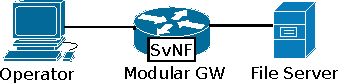
\includegraphics[width=0.30\textwidth]{fig/testbed.pdf}
  \end{center}
  \caption{ SvNF Performances testbed
    \label{fig:testbed}
  }
\end{figure}	


\begin{figure*}
  \begin{center}
    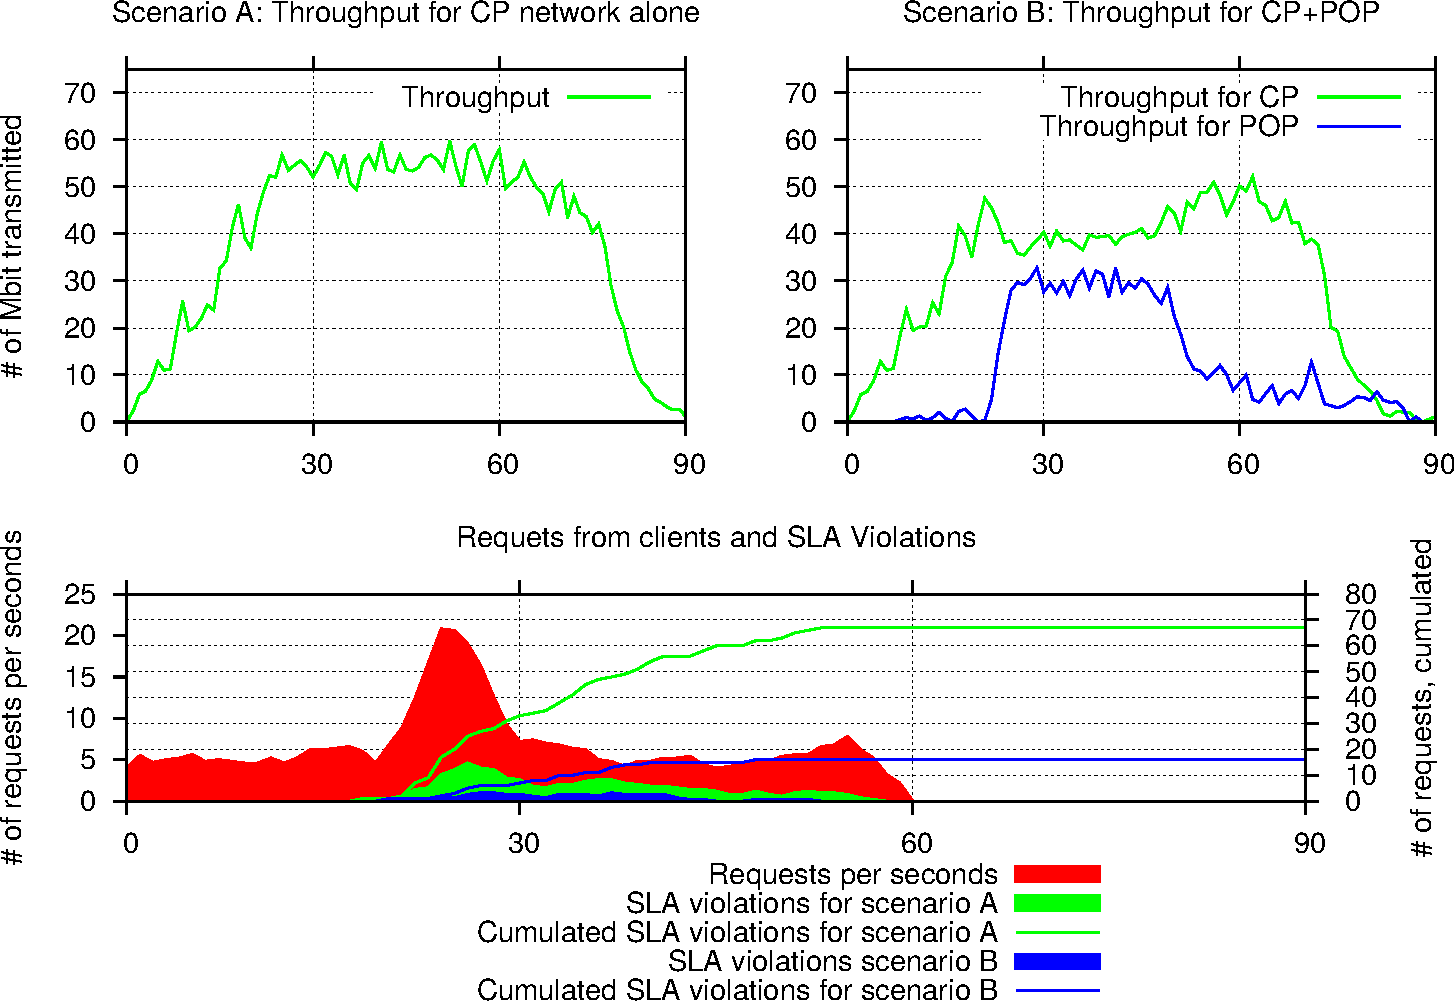
\includegraphics[width=0.95\textwidth]{fig/CP+POP_evaluation.pdf}
  \end{center}
  \caption{ Evaluation of the benefits of the SvNF+vNF system
    \label{fig:cppopeval}
  }
\end{figure*}	







JMeter\footnote{http://jmeter.apache.org} was used to capture the network metrics of our solution.
It allowed us to create agents and make them perform standard HTTP queries and report on specific performances metrics. Each experiment consisted of 10 agents continuously downloading target resources on the HTTP file server, 10000 times.

We considered two different validation usecase: Web Traffic and File Transfer. First, the agents were to download a 192 Mb video file, then a single HTML page which linked to 171 static resources composed of Javascript files, CSS and images of average size 16 kb.

We evaluated our solution with two different rules settings deployed in the SvNF. In the first one, we didn't deploy any rule, assessing only the overhead linked to the application network framework. In the second one however, we deployed 10.000 rules, causing the SvNF to process both requests and responses wrt those rules thereby assessing its ability to perform pattern matching in a timely manner. Both cases reflect the no operation scenario presented in ~section \ref{noop}.

We decided to assess the overhead caused the SvNF by comparing it to the well-known Squid3 HTTP proxy. To have a better grasp of the amont of resources consumed by the SvNF, we also reported CPU and memory consumption for each settings as well.

From ~Table \ref{tab:perf-comparison} we can see that the performances in term of throughput is globally the same across all settings, with the maximum deviation from the baseline settings 1 being less that 0.3\%.
In settings 2-4, we also see that a significant share of CPU power is dedicated to processing the resquests for both Squid3 and the SvNF, with the SvNF consuming up to a 25\% extra CPU time, but with no drop in performances. This can be explained by the fact that the SvNF runs on top of a JVM, while Squid is a native application.

As this experiment doesn't intend to mimic real life internet usages but to stress the system up the its limits, we conclude that even with the extra CPU involved, our solution doesn't significatively penalize the end user, validating that SvNF can be deployed on modular Home Gateways.

\subsection{Simulation of Video Delivery} \label{videodelivery}
\begin{table}
	\scalebox{0.8}{
		\begin{tabular}{| l | l | l|}
		\hline
			\textbf{Settings} & \textbf{Scenario A} & \textbf{Scenario B}\\\hline
			CP Bandwidth &1 Gbps&2 Gbps\\\hline
			POP Bandwidth &0	 Gbps&1 Gbps\\\hline
			POP latency& \multicolumn{2}{l|}{25ms} \\\hline
			CP latency& \multicolumn{2}{l|}{50ms} \\\hline
			Video Distribution& \multicolumn{2}{l|}{Normal} \\\hline
			Video Size&\multicolumn{2}{l|}{Pareto with average video size=10Mb}\\\hline
			Requested bitrate &\multicolumn{2}{l|}{320kbps}\\\hline
			\# of gateways &\multicolumn{2}{l|}{ 200}\\\hline
			\# of video (cruising/peak) &\multicolumn{2}{l|}{ 200/100}\\\hline
			Mean time between request (cruising/peak) &\multicolumn{2}{l|}{ 0.1s/0.05s (Poisson))}\\\hline
			SLA Violation criteria &\multicolumn{2}{l|}{ less than 75\% of the target bitrate 10s after the request}\\\hline
			Video Caching&\multicolumn{2}{l|}{after 4 requests}\\\hline
		\end{tabular}
	}
	\caption{Hypothesis used for simulation\label{simu1}}
\end{table}
We simulated the network deployement presented in ~Figure \ref{fig:hld}, with the specifications presented in ~Table \ref{simu1} with NS3.

We aimed at understanding the benefits for having a POP dynamically provisionning user-requested video. 
The POP beeing located near the user, its latency is reduced wrt the CP network (backed by CDN), hence a possible higher throughput for HTTP traffic like video streaming.
For our simulation, we included two types of patterns. The first one is composed of video requests emmited regularly by the clients, which generate a cruising phase traffic. We also included another source of traffic at \textit{25s} which is caraterized by a greater request arrival rate as well as a more concentrated distribution of videos. Consumption peaks usually occur when a viral video is posted, most of the time on the landing page of the content provider. Beeing able to cache this kind of video and to serve them as close as possible to the users is a key indicator of success for the vNF.

~Figure\ref{fig:cppopeval} depicts two scenarios. In (A) we only rely on CP network to deliver the media while in (B) a single POP is added to the solution. Note that global bandwidth remains the same, as we took some bandwidth from the CP to allocate it to the POP.

We can see that the cruising phase doesn't generate any SLA violation and the CP alone is able to handle the traffic load. However, when the peak occurs, SLA violations increase dramatically, causing a lot of requests to be dropped. In scenario B, however, the presence of the POP as an alternative, low latency data source, mitigate the peak effect and reduces up to 70\% of SLA violations to on the overall simulation period.

Whaving a POP with lower network latency to serve highly redundant requests, benefits to both the user and the content provider. As the former sees an increase in QoS, the latter reduces cost by avoiding the over provisioning of network capabilities. It's important however to reserve POP bandwidth to serve only highly popular videos, so as to maximize its benefits, while keeping the mean latency low between clients and POPs by spreading POPs along the territory.




\subsection{Simulation of provisionning decision} \label{provisionningdecisions}

\begin{figure}
	
 \begin{center}
    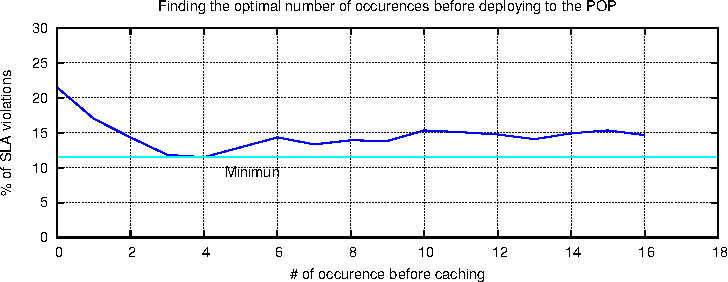
\includegraphics[width=0.45\textwidth]{fig/cachingStrat_evaluation.pdf}
  \end{center}
  \caption{ Caching Strategy Evaluation
    \label{fig:cachingstrateval}
  }
\end{figure}	

POP are designed to have great network performances for a given geographic area, and need to be spread throught the territory for a reduced price.
In order to mitigate the storage cost, the caching controller takes the decision to provision as few videos as possible to fullfill the SLA. Several factor can influence the decision, like the transcoding time, the vNF booting time, hosting costs and so on.
Taking the decision to provision a video in a specific POP means classifying the video as cachable according to some metadata, like the view count in a certain time window.
In \cite{silvestre_boosting_2015}, the authors proposed a model for predicting the popularity of a video, and estimated that view counts accounted for 82\% of the relative importance. 
We implemented a very simple provisionning policy, based on the number of requests for the same resource received in a 10 minutes rolling window. If the number is above the threshold, the video is cached at the POP level and clients can download the video from there.

~Figure \ref{fig:cachingstrateval} shows that for our particular settings, the option that minimize the percentage of SLA violation is 4. This can be explained by the fact that we want to preserve the POP for serving only the most popular videos (which will trigger the most SLA violations) and not clutter it with less popular videos that could be easily served by the CP. However, as the propagation of the caching policy takes time, we want to react promptly and not wait for too many popular videos to hitting the CP.

In production, this evaluation should be updated regularly by monitoring the overall traffic and the network conditions and possibly using other video metadata.







\section{Conclusion and future work \label{sec:conclusion}}

We proposed a solution to help NFV becoming a reality for modular HG, making a first step to a fully virtualized home environment as proposed by ETSI.
We implemented a vNF and we used it to bring major enhancements to the HG, thanks to our SvNF, a small but efficient OSGi bundle, collaborating with vNF deployed in operator POPs.
Other network functions play a key role in virtualizing HG like NAT or DHCP and should also be investigated.
For that, we must solve different issues, more related to network performances than to computational power. 
Further work will investigate the benefits for the CP and SP in having such a SvNF+vNF approach, focusing on the search of a cost function permitting them to take the proper decisions for Caching \& Transcoding processings according to their deployed elements (POPs, CDNs, ...), for instance. 
We will consider alternative execution environements for the Gateway.




\section*{Acknowledgments}
The work performed for this paper has been partially funded by the FP7 IP T-NOVA European Project (Grant Agreement N\degree619520) and the FUI French National Project DVD2C.
\bibliographystyle{IEEEtran}
\bibliography{vnf}





% that's all folks
\end{document}


